\section{Design und Planung}

\subsection{Erstellung des ERDs}
Um zu gewährleisten, dass die Systemanforderung getroffen werden, ist es notwendig ein entsprechendes \gls{erd} zu erstellen.
Innerhalb eines \gls{erd} werden alle verschiedene Entitäten, Attribute sowie deren Beziehungen dargestellt.
Dieses dient als gemeinsamer Nenner für die Projektentwicklung, da jedes Teammitglied eine eigene Vorstellung der Datenstruktur haben könnte. 
Ein weiterer Vorteil eines \gls{erd}s ist das Potenzial Fehlerquellen zu identifizieren und dadurch zukünfige Problem zu umgehen. 

Nach dem die benötigten Entitäten, sowie deren Attribute festgelegt wurden, müssen nun die Beziehungen zwischen ihnen festgelegt werden. 
Dabei wird gewählt zwischen One-to-One, One-to-Many und Many-to-Many Beziehungen, wobei die Many-to-Many Beziehung innerhalb einer Assoziationstabelle dargestellt wird. 

Innerhalb dieser Arbeit ist die Entität \emph{Exhibitions} das zentrale Objekt, dies ist in den Abbildung \ref{fig:erd:lastversion} gut ersichtlich.
Die Beziehungen zwischen \emph{Positionen, Exhibits, Rooms und Exhibitions} stellt sich besonders als Herausforderung dar, aufgrund der vielen Abhängigkeiten untereinander. 

Üblicherweise muss das \gls{erd} im Laufe der Entwicklung etwas überarbeitet werden. 
Unsere Gründe dafür waren einige Planänderungen bei der Kommunikation zwischen zwei Entitäten, sowie der Aufbau der Hauptentitäten \emph{Exhibition und Exhibit} (siehe Abb. \ref{fig:erd:firstversion}).

 
\begin{figure}
    \centering
    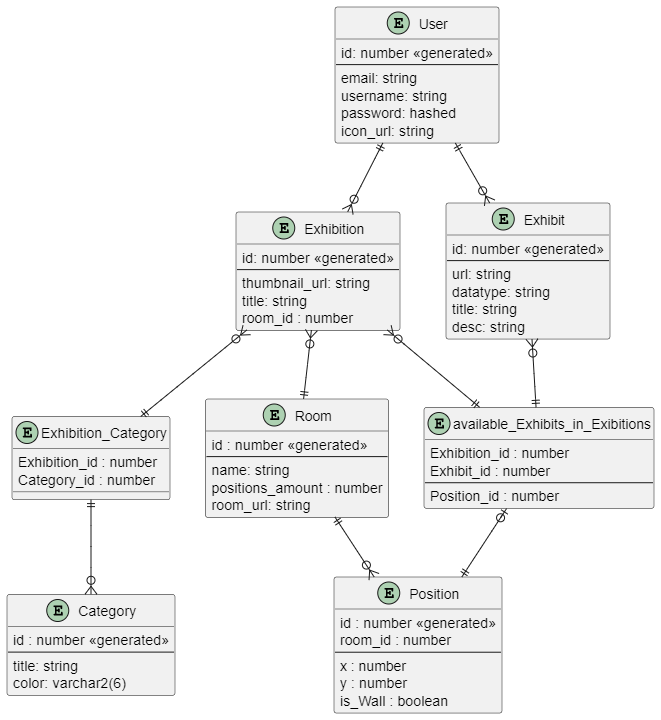
\includegraphics[scale=0.5]{pics/firstversion_erd.png}
    \caption{Erste Version des ERDs}
    \label{fig:erd:firstversion}
\end{figure}

\begin{figure}
    \centering
    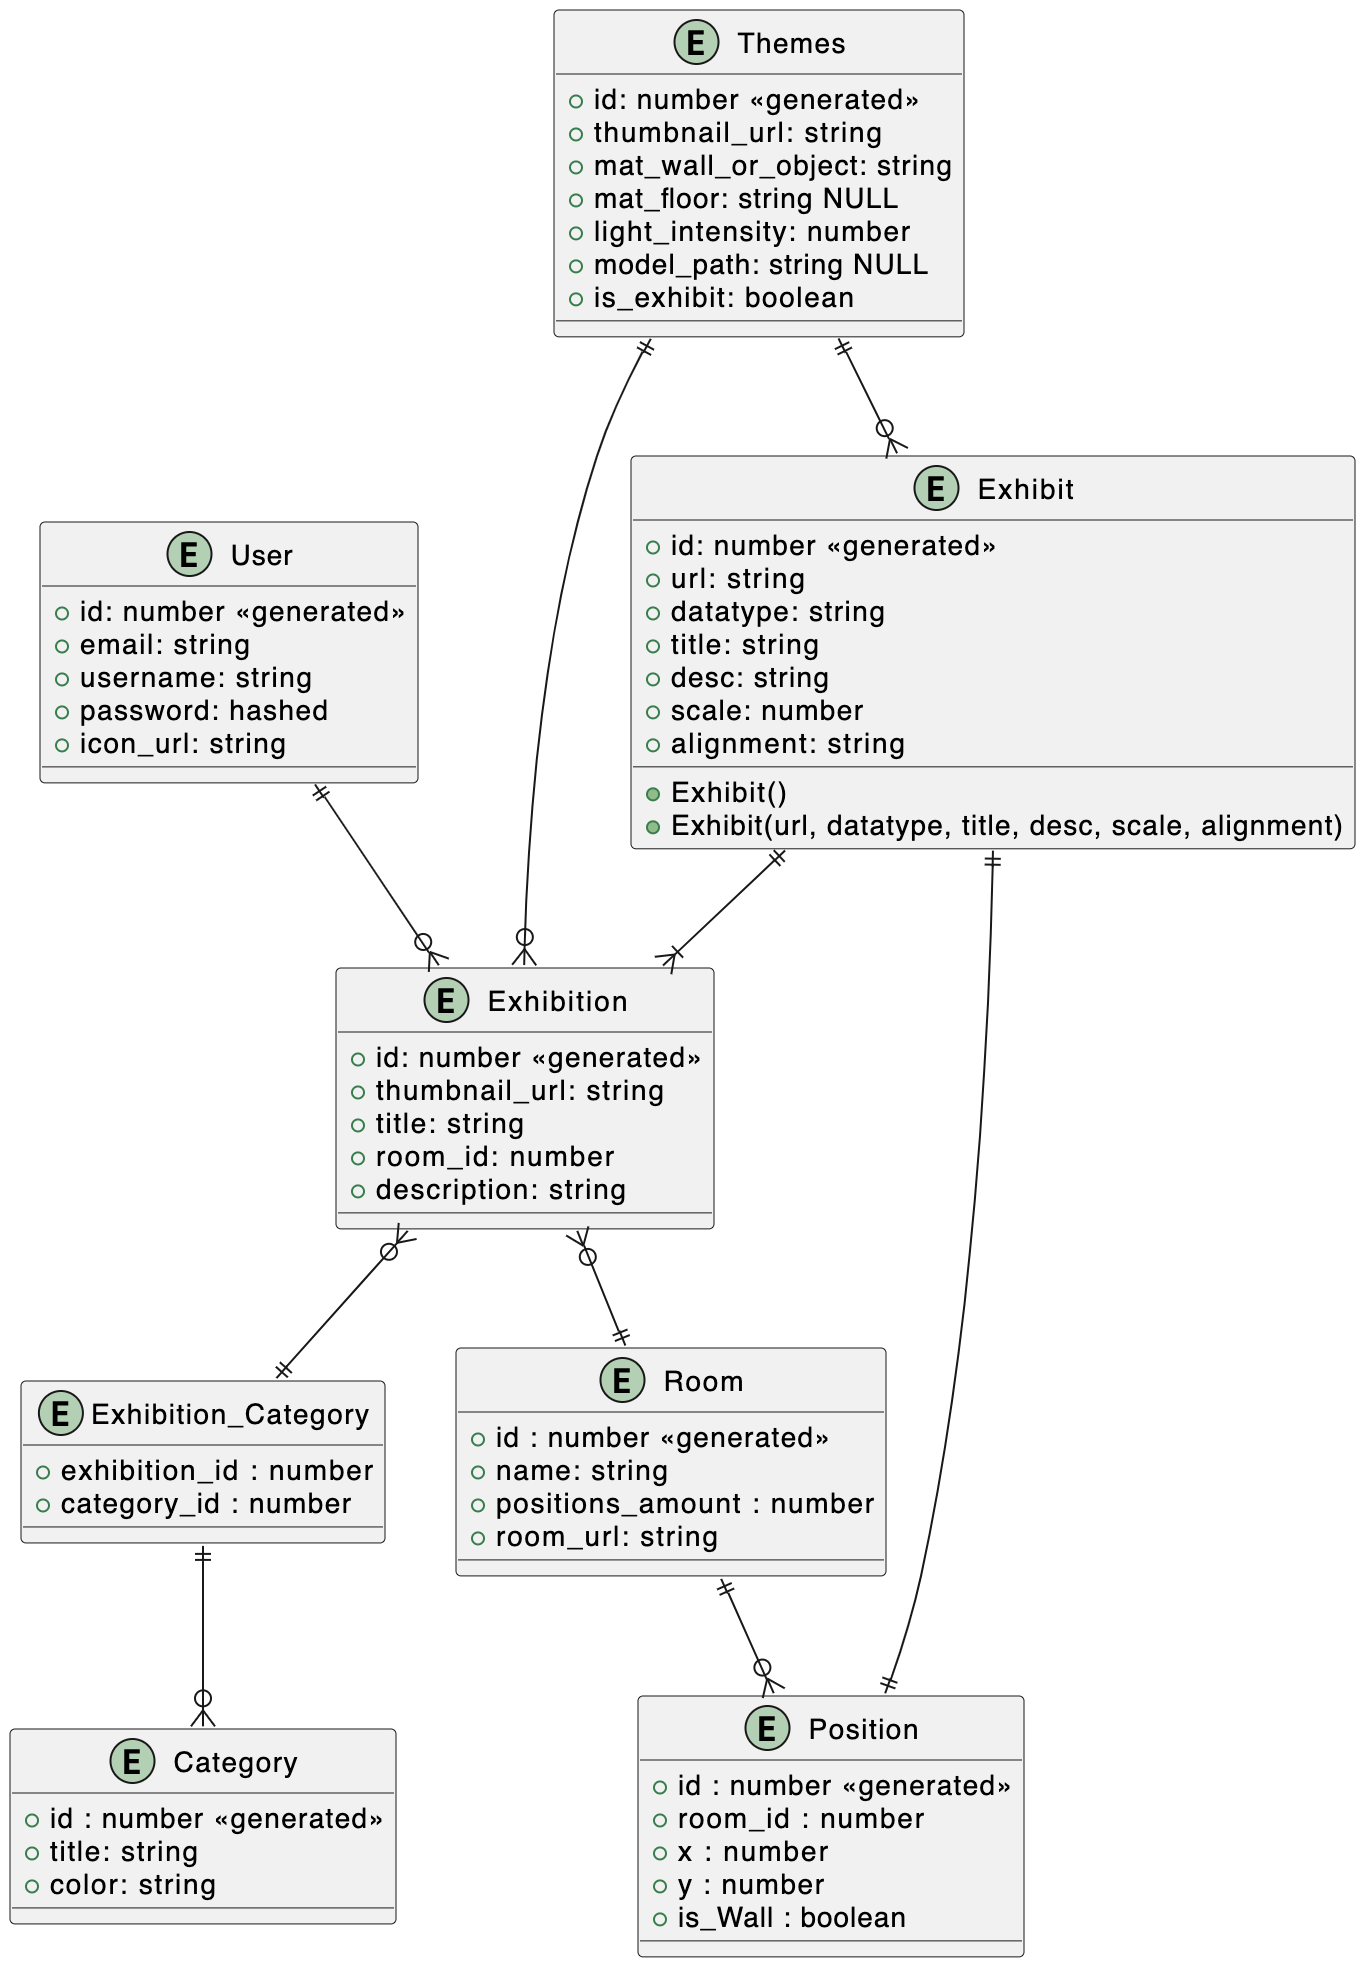
\includegraphics[scale=0.5]{pics/lastversion_erd.png}
    \caption{Finale Version des ERDs}
    \label{fig:erd:lastversion}
\end{figure}

\section{Aufsetzen der Datenbank und des Servers}

\subsection{Umsetzung des ERDs in Quarkus}
Bevor das \gls{erd} umgesetzt werden kann, muss ein Quarkus Projekt erstellt werden, und PostgreSQL lokal gestartet werden. 
Das erste Ziel ist es, das Projekt lokal starten zu können und eine Datenbankverbindung herzustellen. 
Um ein Quarkus Projekt zu erstellen wurde das Quarkus Plugin von JetBrains s.r.o. verwendet. 
Hiermit werden die Funktionen der Webseite \href{https://code.quarkus.io}{code.quarkus.io} in einem IntelliJ Fenster dargestellt (siehe Abb. \ref{fig:intellij:plugin}). 

\begin{figure}
    \centering
    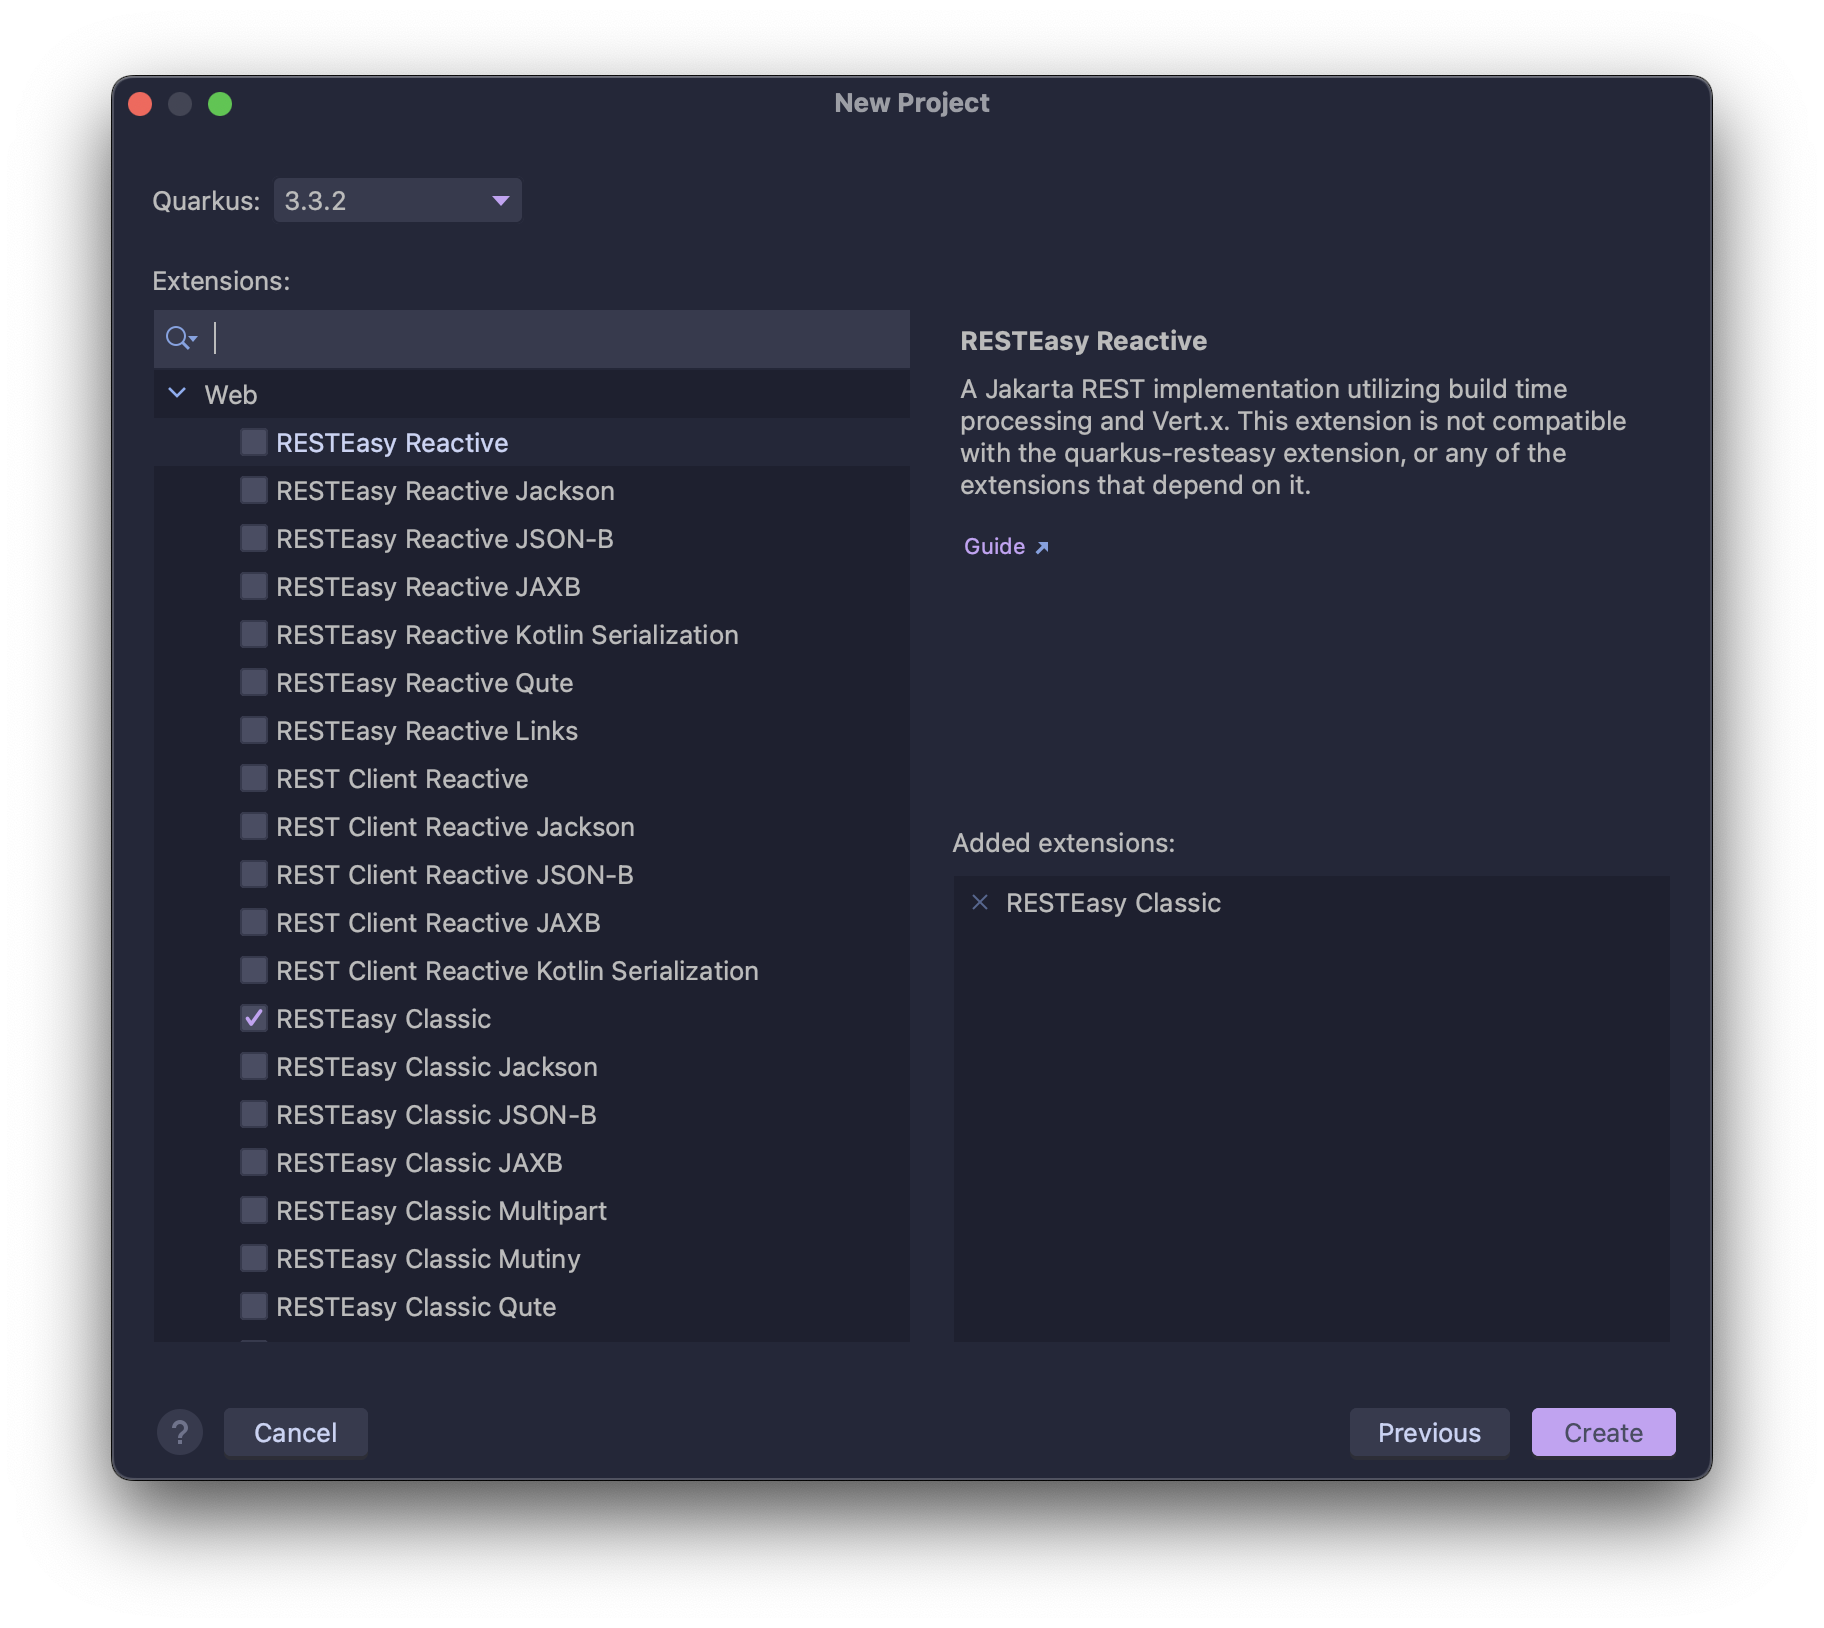
\includegraphics[scale=0.4]{pics/quarkusplugin.png}
    \caption{Auswählen der gewünschten Quarkus Extensions im Quarkus Plugin}
    \label{fig:intellij:plugin}
\end{figure}

Als nächstes wird eine Verbindung zur lokalen Datenbank aufgebaut. 
Dafür werden die Konfigurationen in Abb. \ref{lst:quarkusDatasourceProject} benötigt.

\begin{lstlisting}[label=lst:quarkusDatasourceProject]
    quarkus.datasource.db-kind=postgresql
    quarkus.datasource.username = postgres
    quarkus.datasource.password = postgres
    quarkus.datasource.jdbc.url=jdbc:postgresql://localhost:5432/postgres

    quarkus.hibernate-orm.database.generation=drop-and-create
\end{lstlisting}

Falls der Verbindungsaufbau versagt, wirft Quarkus während der Kompilierung Fehlermeldungen. 
Ansonsten können nun die Tabellen angelegt werden. 
Diese lassen sich mittels der Annotation \emph{@Entity} definieren. 
Durch die Entwicklung mithilfe des Hibernate \gls{orm} mit Panache brauchen die einzelnen Klassen keine explizit definierte Id, sondern nur die Extensioins der \emph{PanacheEntity}-Klasse (siehe Abb. \ref{lst:exhibitionEntityCode}, Zeile2). 

Beziehungen werden durch die Annotationen \emph{@OneToMany, @ManyToMany, @OnetoOne} dargestellt. 
Jede Beziehung muss auf einer Seite gemapped werden, da sie sonst mehrfach generiert wird(siehe Abb. \ref{lst:exhibitionEntityCode}, Zeile 4). 
Bei Many-to-Many wird eine zuätzliche Annotation @JoinTable hinzugefügt, um die Assoziationstabelle zu konfigurieren (siehe Abb. \ref{lst:exhibitionEntityCode}, Zeilen 5 bis 12). 
Zu den Relationen können zusätzlich noch \gls{cascade} festgelegt werden. 

\begin{lstlisting}[label=lst:exhibitionEntityCode, language=java]
@Entity
public class Exhibition extends PanacheEntity {
    // ...
    @OneToMany(mappedBy = "exhibition", cascade = CascadeType.REMOVE)
    public List<Exhibit> exhibits;

    @ManyToMany
    @JoinTable(
            name = "exhibitions_categories",
            joinColumns = @JoinColumn(name = "exhibition_id"),
            inverseJoinColumns = @JoinColumn(name = "category_id")
    )
    public Set<Category> categories;
}
\end{lstlisting}

Für die Entitäten Theme, Positionen und Rooms hat sich das Team dafür entschieden, die Daten vorgefertigt in die Datenbank zu laden. 
Das bedeutet, dass für diese Entitäten keine Methoden angelegt werden müssen, um neue Objekte zu erstellen. 
Verwendet wurde dafür eine \emph{import.sql}-Datei. 
Diese wird bei jedem Quarkus Start ausgeführt. 

\subsection{Implementierung der REST-Schnittstellen}

Um das Frontend auf die Daten zugreifen zu lassen werden Schnittstellen benötigt, die dies ermöglichen. 
Dafür werden im Backends Resource-Klassen erstellt, um die einzelnen Endpoints zu verwalten. 
Diese definiert man durch die \emph{@Path}-Annotation, da diese angibt, unter welchem Pfad die Methoden erreichbar sind. 
Für jede Methoden muss zusätzlich die \gls{http}-Methode als Annotation definiert werden. 

\subsubsection{Repositories} 
Um in Resource-Klassen die Datenbank anzusprechen, müssen die benötigten Repositories injiziert werden. 
Durch die Verwendung der Panache Extension, implementieren alle Repository-Klassen das \emph{PanacheRepository}, wobei die zugehörige Tabelle in spitzen Klammern angegeben werden muss, wie in Code Beispiel \ref{lst:panacherepo} bei Zeile 2.
Dieses fügt einfache Methoden für \gls{crud}-Operationen hinzu, ohne diese zusätzlich zu definieren. 

\begin{lstlisting}[label=lst:panacherepo, language=Java, caption=Teil aus dem Exhibition Repository]
@ApplicationScoped
public class ExhibitionRepo implements PanacheRepository<Exhibition> {
    //...
    public List<ExhibitionWithUserRecord> listAllExhibitionsWithUserField() {
        String sql = "select new 
            org.threeDPortfolioGallery.records.ExhibitionWithUserRecord(e, u.user_name, u.icon_url) from Exhibition e join e.user u left join e.categories c";
        TypedQuery<ExhibitionWithUserRecord> q = getEntityManager()
                .createQuery(sql, ExhibitionWithUserRecord.class);
        var ret = q.getResultList();
        return ret;
    }
}
\end{lstlisting}

Die Repositories ermöglichen ebenso das Definieren von eigenen \gls{jpql}-Befehlen. 
\gls{jpql} ermöglicht, neben der Nutzung der gewohnten \gls{sql}-Keywords, das definieren von Parametern in Queries, sowie die Verwendung von eigenen Records und \gls{dto}s.

\subsubsection{Records und DTOs}
Records sind eine Möglichkeit, einen Datensatz zurückzugeben, mit Werten aus verschiedenen Tabellen. 
Sie können gesetzt werden, jedoch nicht mehr geändert werden. 
Deswegen eignen sie sich besonders gut, Daten aus \gls{sql}-Statements zu speichern und zu returnen.

\gls{dto}s hingegen können mittels Set-Methoden die Werte wieder ändern.
Dies ist nicht umbedingt notwendig beim Auslesen der Datenbank, aber sehr nützlich beim Anlegen neuer Objekte. 

\subsubsection{User}
Ein User wird angelegt durch das Definieren eines Nutzernamens, sowie eines Passwortes. 
Optional können ebenso Pfade angegeben werden für Profilbilder. 
Jedes Passwort bekommt vor dem Speichervorgang einen Salt angehängt und wird mithilfe von Base64 verschlüsselt. 

Der Zugriff auf die Schnittstelle ist gesichert durch ein Tokensystem. 
Nach jedem erfolgreichem login wird ein Token zurückgesendet, der für die Authentifizierung genutzt werden kann. 
In diesem Token ist der Nutzername gespeichert, sowie zu welcher Gruppe der Nutzer angehört. 
Je nach Gruppe kann auf verschiedene Endpoints zugegriffen werden. 
Die Limitationen werden bei der Definition der Methoden angegeben mittels \emph{@PermitAll}, was keine Limitationen hinzugefügt.
Genauso gibt es jedoch \emph{@RolesAllowed}, was nur definierten Rollen den Zugriff erlaubt.  


\subsubsection{Exhibitions}
Eine der wichtigsten Funktionen der Exhibitions-Resource, ist das Anlegen einer Exhibition. 
Dafür wird eine \emph{@POST}-Methode erstellt, die ein Objekt nach dem \gls{dto} in Codeausschnitt \ref{lst:exhibitiondto} einliest.
\gls{dto}s können auch verschachtelt werden, was in Zeile 12 erkennbar ist. 

In der Klasse wurde ebenfalls die Annotation \emph{@Data} verwendet. 
Diese stammt aus der Java Library Project Lombok und automatisiert die erstellung von Get- und Set-Methoden. 
\cite{Lambok}

\begin{lstlisting}[label=lst:exhibitiondto, language=Java, caption=Exhibition DTO]
    @Data
    public class AddExhibitionDTO {
        String thumbnail_url;
        String title;
        String description;

        Long room_id;

        Long user_id;
        Long[] category_ids;

        AddExhibitDTO[] exhibits;
    }
\end{lstlisting}

Da die Methode ein \gls{dto} erwartet, muss definiert werden, dass etwas eingelesen werden soll. 
Dies macht man durch das \emph{@Consumes}. 
Der Codeabschnitt \ref{lst:newExhibitionMethod} Zeile 4 legt fest, dass beim Senden der POST-Methode ein \gls{json}-Objekt erwartet werden soll. 
Der Ausdruck in der Klammer in Zeile 5 im selben Abschnitt beschreibt, wie dieses Objekt konstruiert sein soll.

Beim Aufruf der Methode wird das mitgegebene Objekt in der Variable \emph{newExhibition} gespeichert.
Danach werden zwei leere Variable initialisert. 
Zum einen eine neue Exhibition, zum anderen eine LinkedList bestehend aus Exhibits.
Diese sind getrennt, da alle Exhibits zuerst in die Datenbank eingefügt werden müssen, bevor die Exhibition tatsächlich gespeichert wird. 

Neben den Exhibits, müssen genauso die anderen Werte der mitgegebenen Variable geprüft werden. 
Das heißt, es muss sichergestellt werden, dass keine nicht-existierenden User- oder Category-Ids übergeben wurden. 
Falls etwas einen Fehler während der Überprüfung wirft, Fehlermeldung zurückgegeben mit dem Statuscode 406 "Not Acceptable". 
Gleichzeitig geschieht ein Rollback der davor gespeicherten Objekte. 
Diese Vorgehensweise wird durch die Annotation \emph{@Transactional} definiert. 

\begin{lstlisting}[label=lst:newExhibitionMethod, language=Java, caption=Methode zum Anlegen von Exhibitions]
    @POST
    @Transactional
    @Path("/new")
    @Consumes(MediaType.APPLICATION_JSON)
    public Response postNewExhibition(AddExhibitionDTO newExhibition){
        Exhibition exhibition = new Exhibition();
        List<Exhibit> newExhibitList = new LinkedList<>();
        // ...
    }
\end{lstlisting}

\subsubsection{Filemanagement}
Der File-Upload geschieht während der Bearbeitung der Exhibition im Frontend. 
Nach jeder Dateiauswahl des Nutzers der Webseite, wird der Endpoint zuständig für den Fileupload aufgerufen. 
Dieser erwartet sich, anders als die anderen POST-Methoden, kein \gls{json}-Objekt, sondern eine Datei. 
Wiedermals wird dies fesgelegt mittels der \emph{@Consumes}-Annotation, mit \emph{"multipart/form-data"} als Wert. 
Das Limit der akzeptierten Datein wird in den \emph{application.properties} (Abb. \ref{lst:filesizemax}) festgelegt. 
\begin{lstlisting}[label=lst:filesizemax]
    quarkus.http.limits.max-body-size = 300m
\end{lstlisting}

Für das eigentliche Abspeichern einer Datei, ist die Methode \emph{writeFile()} zuständig (siehe Abb. \ref{lst:fileupload}). 
Diese wird aufgerufen, wenn der Endpoint aufgerufen wird und eine Datei mitgegeben wurde. 
Der erste Parameter der Methode, das Byte-Array, wird mittels eines Inputstreams erstellt. 
Der Filename wird in einer extra Methode erstellt. 
Dafür wird der ursprüngliche Name der Datei genommen und untersucht auf Leerzeichen. 
Sobald diese entfernt wurden, wird der abgeänderte Name zurückgegeben. 

Nachdem das File abgespeichert wurde, wird dessen Pfad mit dem neuen Namen in die Response mitgegeben. 
Diese Antwort wird dann als Wert erwartet als Url, beim Anlegen neuer Exhibits. 

%  POST-Methode der Exhibition aufgerufen wird. 
% Da jedes Exhibit eine Datei beinhaltet muss diese hochgeladen werden, um den Abruf ohne fehlende Daten zu ermöglichen.

\begin{lstlisting}[label=lst:fileupload, language=Java, caption=Hochladen der Dateien]
    private void writeFile(byte[] content, String filename) throws IOException {
        File file = new File(filename);
        if (!file.exists()) {
            file.createNewFile();
        }
        FileOutputStream fos = new FileOutputStream(file);
        fos.write(content);
        fos.flush();
        fos.close();
    }
\end{lstlisting}



\section{Hosten auf einer Cloud}

\section{Schreiben der Tests}

%TODO das wegmachen, for safety bleibt das noch drinnen
next termin:
    fertig mit praktischem dienstag 6. EH (12:45) am 3.10 treffen beim eingang
    sonntag abend immer schicken

feedback:
- weglassen von der anfangsfrage
- umsetzung gliedern nach user stories